\section{SISTEMA INTEGRADO: Implementación}

\subsection{Introducción}

El objetivo de este trabajo era proponer un nuevo sistema de control baso en lógica difusa y redes neuronales convolucionales para que el robot pueda tomar mejores decisiones a la hora de sortear un obstáculo, para esto el modulo de procesamiento de imágenes y el modulo de lógica difusa detallados anteriormente trabajaran en conjunto para una mejor toma de decisión sobre una placa de desarrollo Zybo-Z7 y s.\par
A su vez para probar el sistema de control propuesto se llevo a cabo la construcción de un robot.

\subsection{Hardware y elementos utilizados}


\begin{figure}[htbp]
\centering
\quad
\subfigure[Zybo-z7 x1]{
\begin{minipage}[t]{0.25\linewidth}
\centering
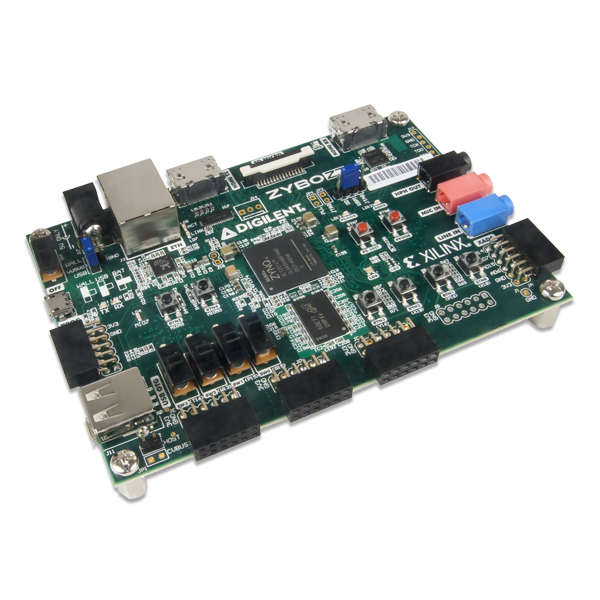
\includegraphics[width=1in]{Tesis/Capitulos/05_CAPITULO_3/img/zybo-z7-0.png}
%\caption{fig1}
\end{minipage}%
}%
\quad
\subfigure[Modulo ov7670 x1]{
\begin{minipage}[t]{0.25\linewidth}
\centering
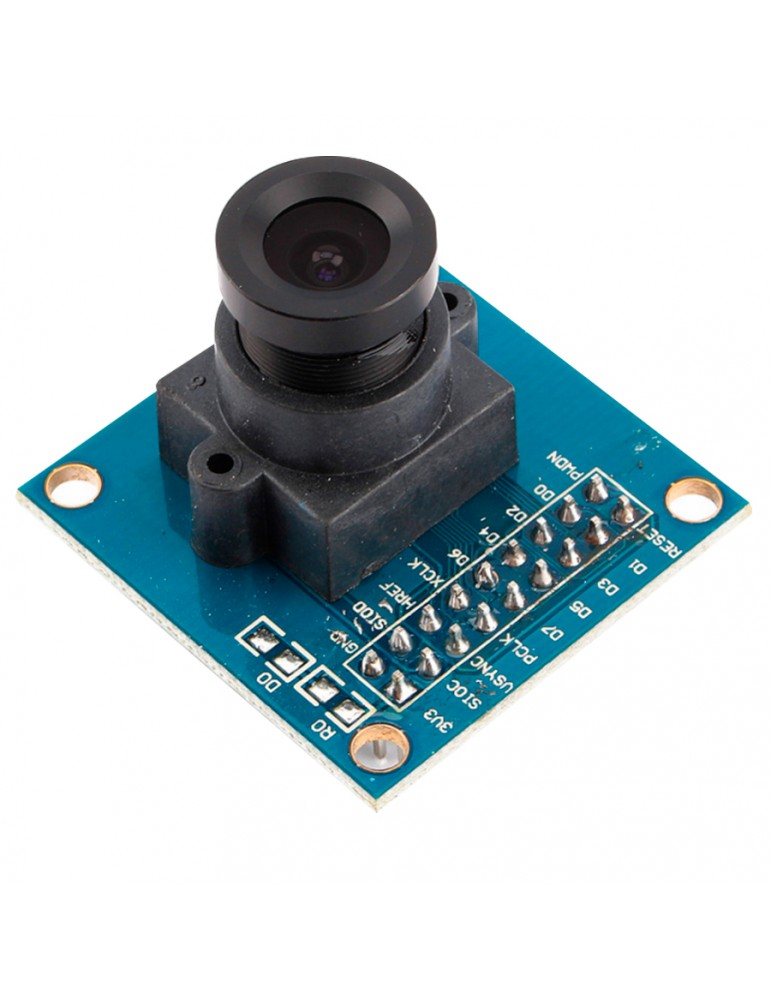
\includegraphics[width=1in]{Tesis/Capitulos/05_CAPITULO_3/img/modulo-camara-ov7670.jpg}
%\caption{fig2}
\end{minipage}%
}%
\quad
\subfigure[Protoboard x1]{
\begin{minipage}[t]{0.25\linewidth}
\centering
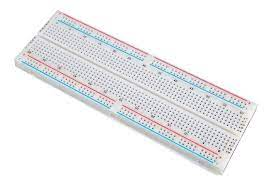
\includegraphics[width=1in]{Tesis/Capitulos/05_CAPITULO_3/img/proto.jpeg}
%\caption{fig2}
\end{minipage}
}%
\subfigure[Hc-sr04 x3]{
\begin{minipage}[t]{0.25\linewidth}
\centering
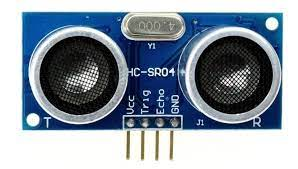
\includegraphics[width=1in]{Tesis/Capitulos/05_CAPITULO_3/img/sr04.jpeg}
%\caption{fig2}
\end{minipage}
}%
\quad
\subfigure[Cables]{
\begin{minipage}[t]{0.25\linewidth}
\centering
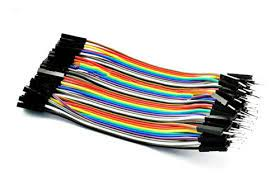
\includegraphics[width=1in]{Tesis/Capitulos/05_CAPITULO_3/img/cables.jpeg}
%\caption{fig2}
\end{minipage}
}
\subfigure[FC-03 encoder x2]{
\begin{minipage}[t]{0.25\linewidth}
\centering
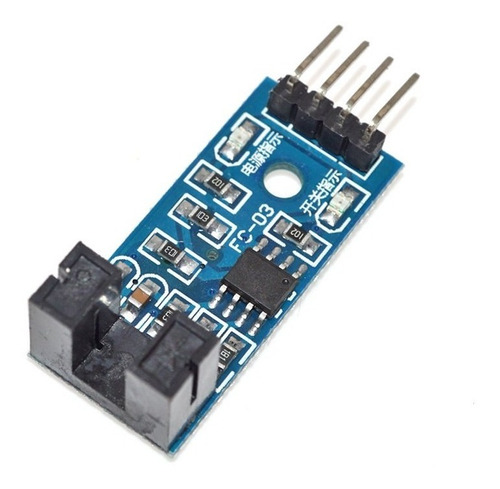
\includegraphics[width=1in]{Tesis/Capitulos/05_CAPITULO_3/img/FC-03.jpg}
%\caption{fig2}
\end{minipage}
}
\quad
\subfigure[Estructura de robot x1]{
\begin{minipage}[t]{0.25\linewidth}
\centering
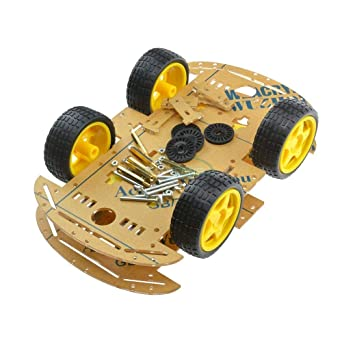
\includegraphics[width=1in]{Tesis/Capitulos/05_CAPITULO_3/img/kitcar.jpg}
%\caption{fig2}
\end{minipage}
}
\quad
\subfigure[l298n x1]{
\begin{minipage}[t]{0.25\linewidth}
\centering
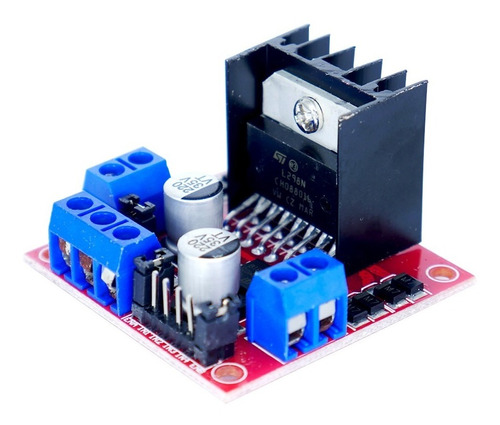
\includegraphics[width=1in]{Tesis/Capitulos/05_CAPITULO_3/img/L298n.jpg}
%\caption{fig2}
\end{minipage}
}
\quad
\subfigure[mini360 x1]{
\begin{minipage}[t]{0.25\linewidth}
\centering
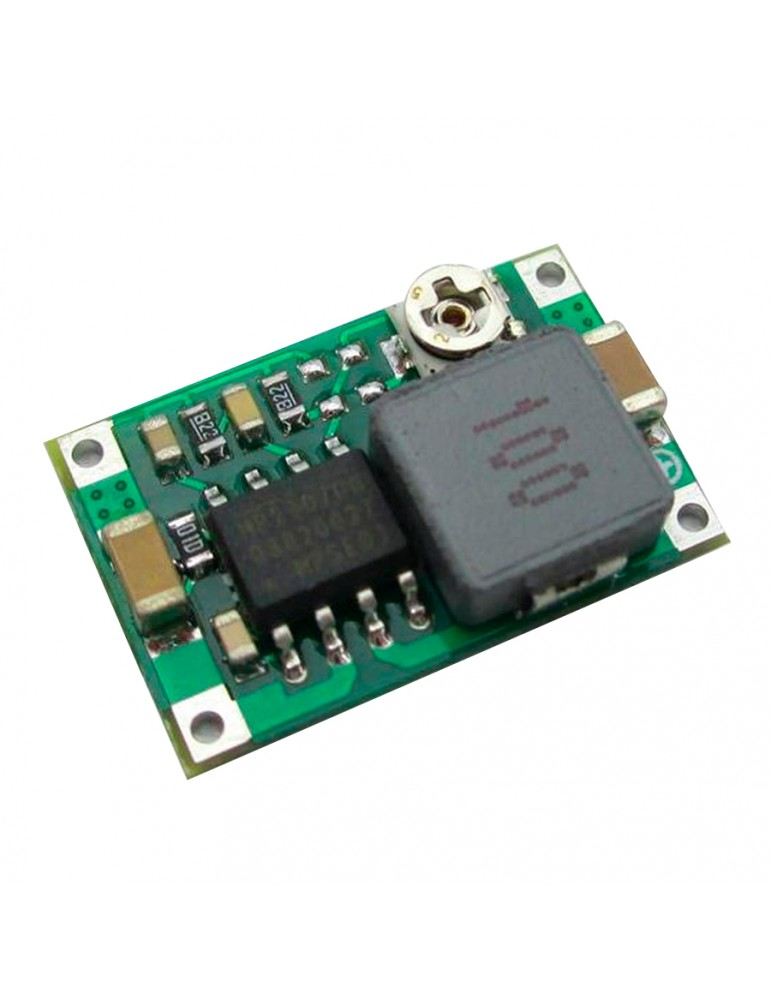
\includegraphics[width=1in]{Tesis/Capitulos/05_CAPITULO_3/img/mini360.jpg}
%\caption{fig2}
\end{minipage}
}
\quad
\subfigure[qmc5883l x1]{
\begin{minipage}[t]{0.25\linewidth}
\centering
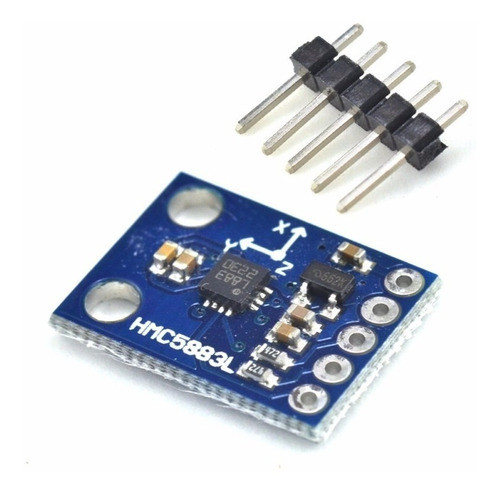
\includegraphics[width=1in]{Tesis/Capitulos/05_CAPITULO_3/img/Qmc5883l.jpg}
%\caption{fig2}
\end{minipage}
}
\quad
\subfigure[porta baterias 18650 x2]{
\begin{minipage}[t]{0.25\linewidth}
\centering
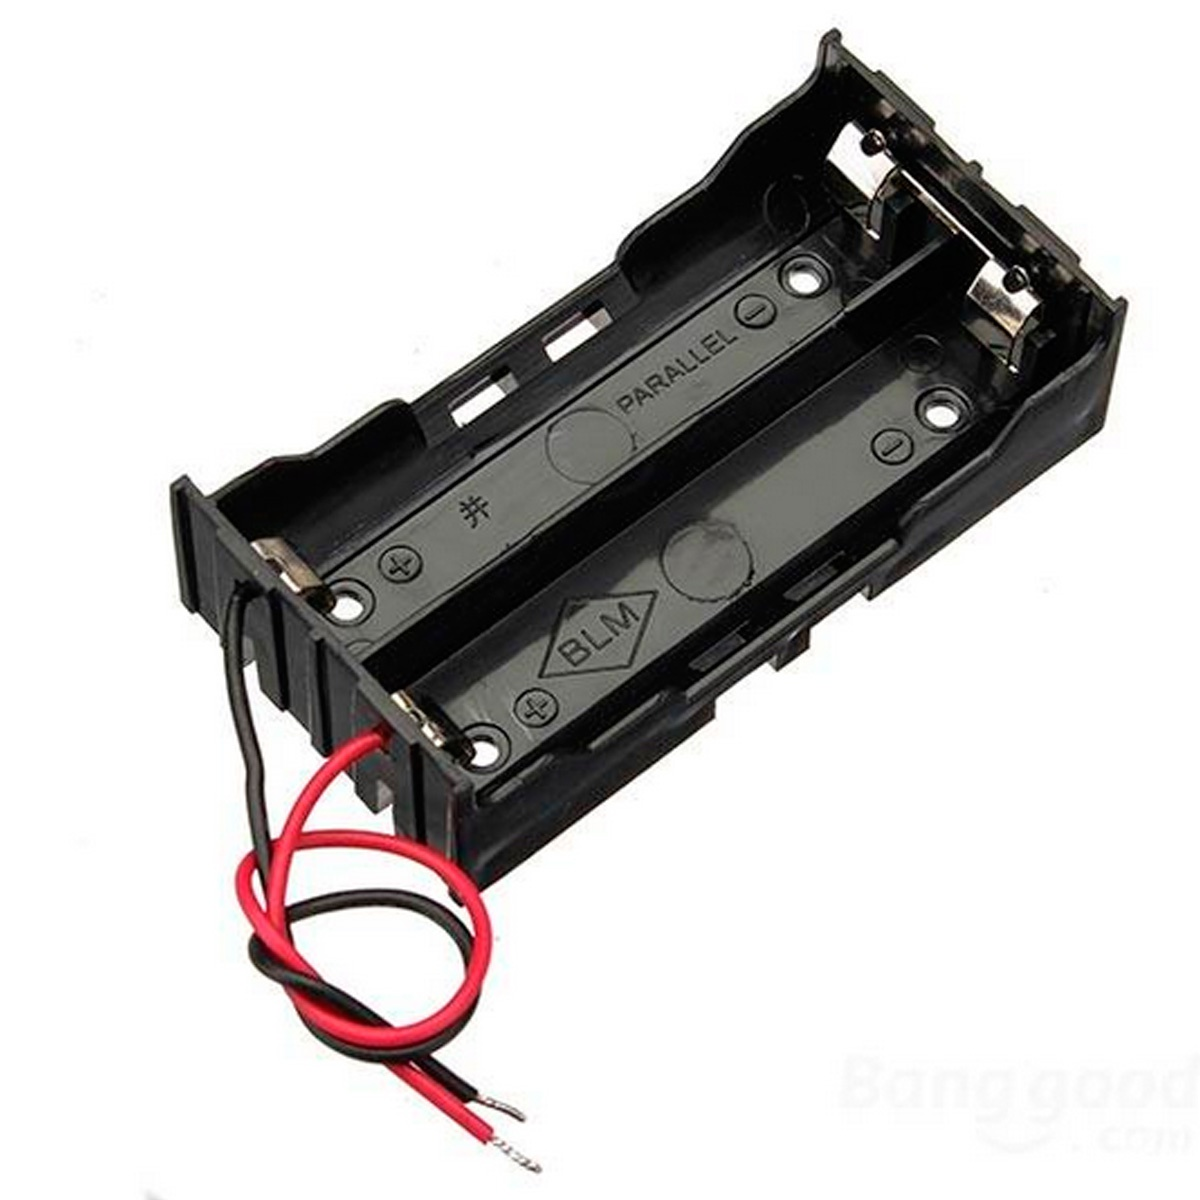
\includegraphics[width=1in]{Tesis/Capitulos/05_CAPITULO_3/img/portabaterias.jpeg}
%\caption{fig2}
\end{minipage}
}
\quad
\subfigure[Baterias 18650 x4]{
\begin{minipage}[t]{0.25\linewidth}
\centering
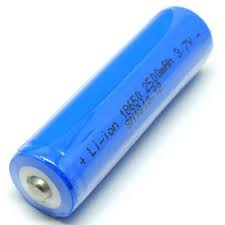
\includegraphics[width=1in]{Tesis/Capitulos/05_CAPITULO_3/img/18650.jpeg}
%\caption{fig2}
\end{minipage}
}
\centering
\caption{Elementos y hardware}
\end{figure}

\subsection{Armado y construcción de la plataforma para testear el sistema de control propuesto}


\begin{figure}[htbp]
\centering
\quad
\subfigure[Estado 1]{
\begin{minipage}[t]{0.25\linewidth}
\centering
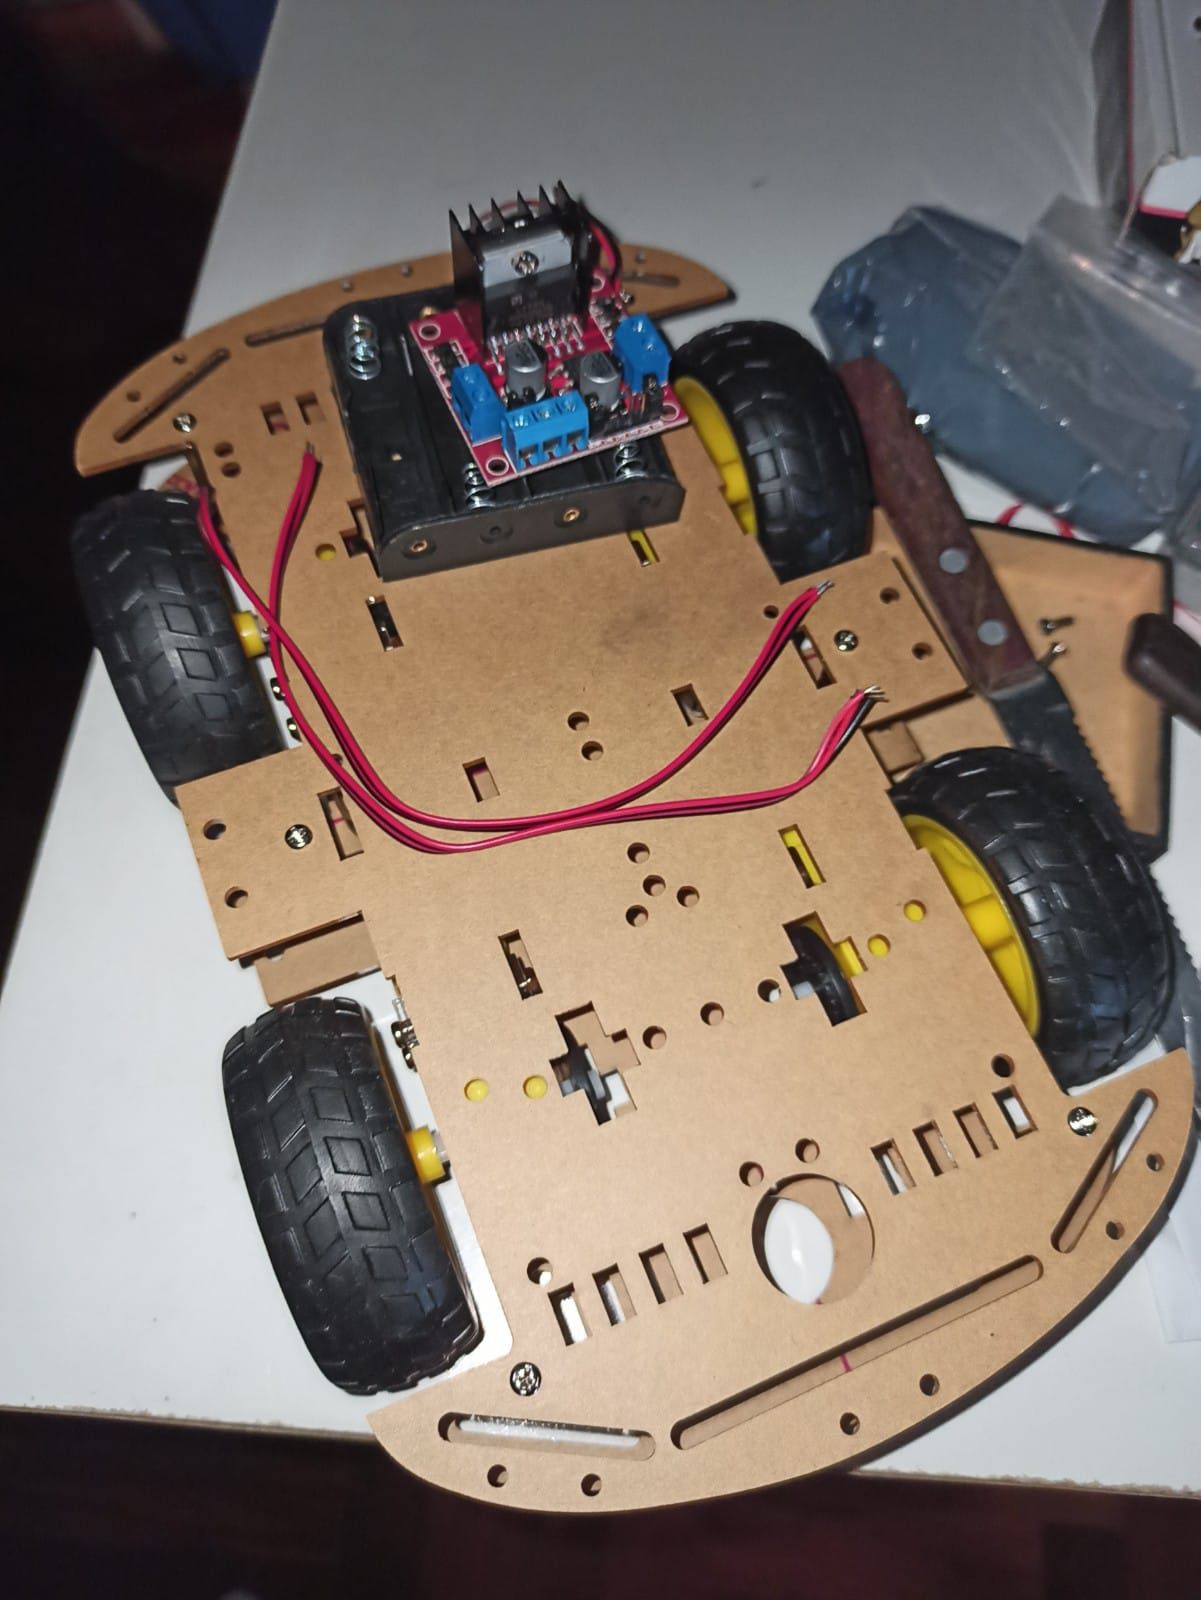
\includegraphics[width=1.5in]{Tesis/Capitulos/05_CAPITULO_3/img/state1.jpeg}
%\caption{fig1}
\end{minipage}%
}%
\quad
\subfigure[Estado 2]{
\begin{minipage}[t]{0.25\linewidth}
\centering
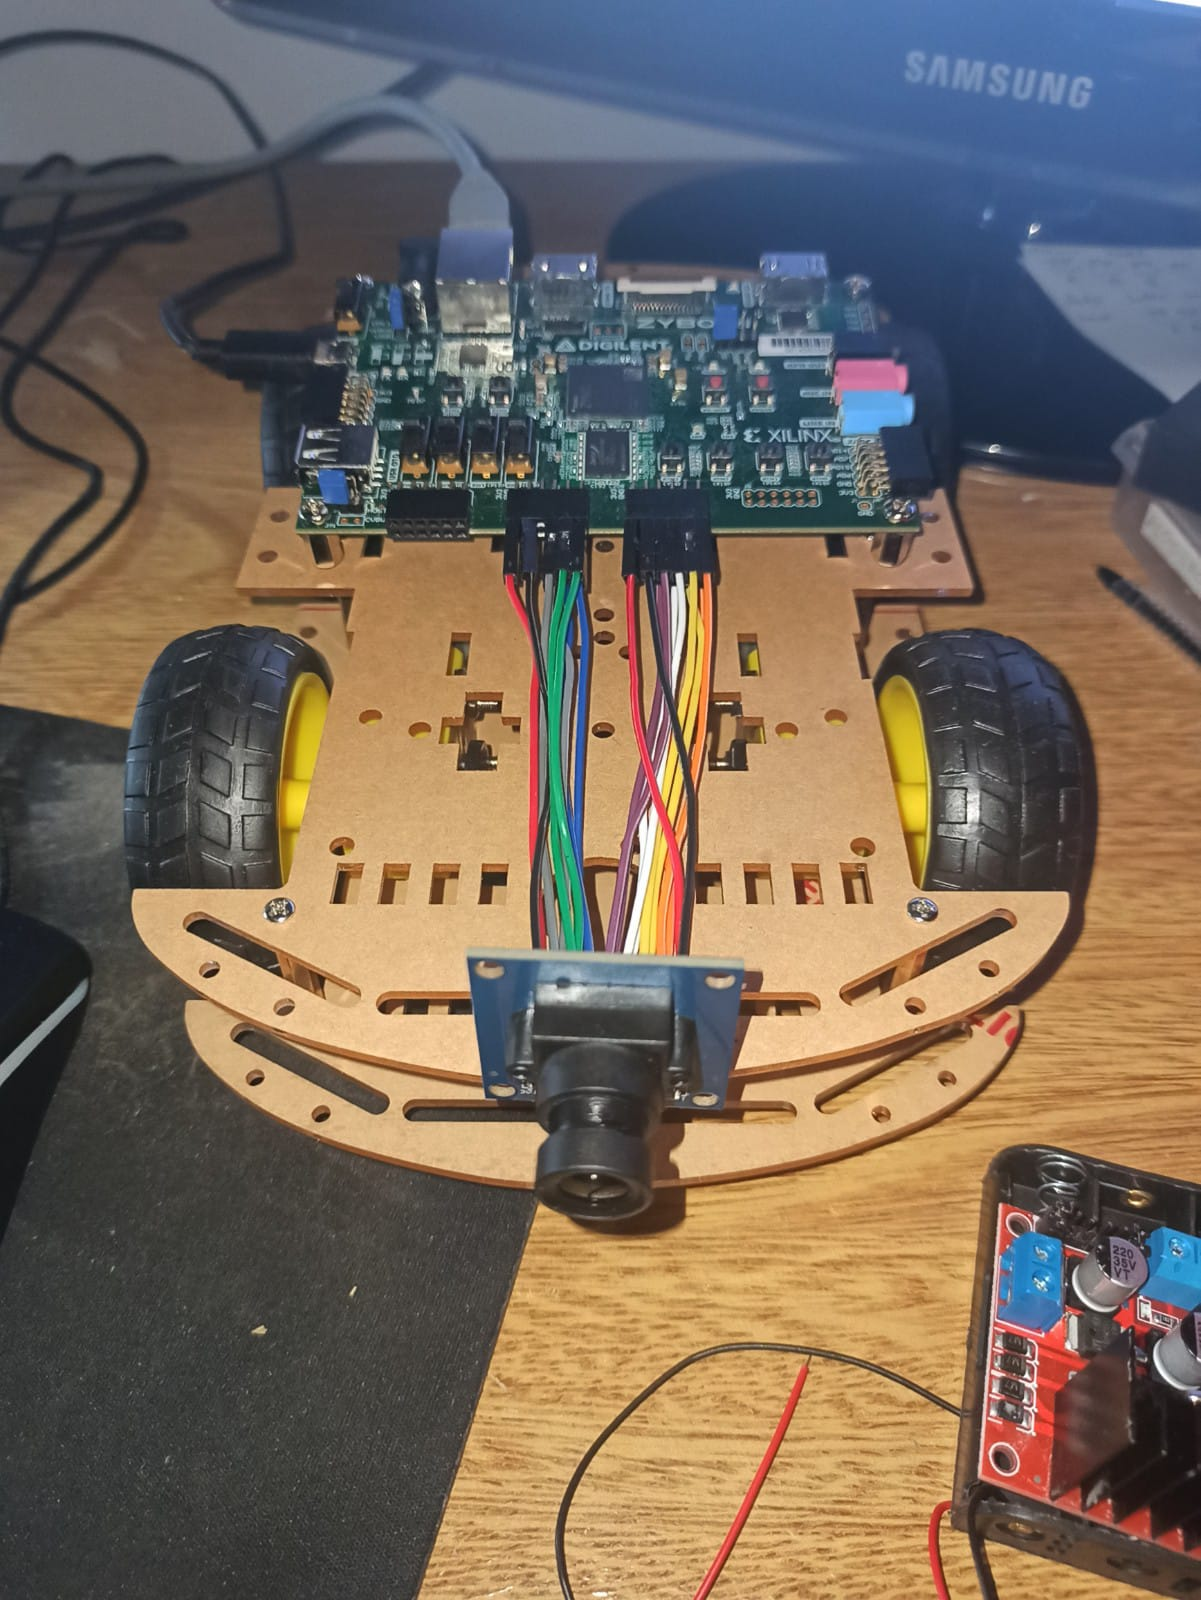
\includegraphics[width=1.5in]{Tesis/Capitulos/05_CAPITULO_3/img/state4.jpeg}
%\caption{fig2}
\end{minipage}%
}%
\quad
\subfigure[Estado 3]{
\begin{minipage}[t]{0.25\linewidth}
\centering
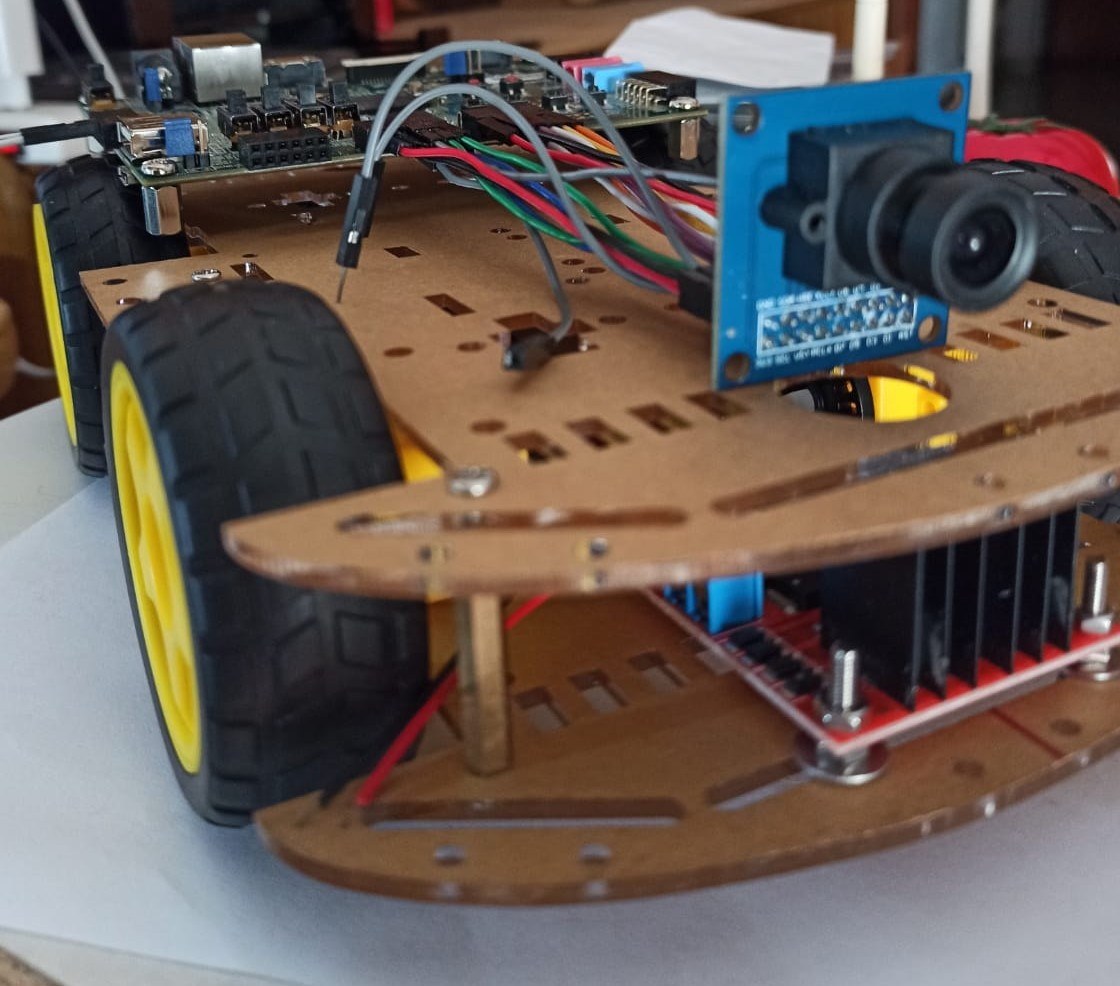
\includegraphics[scale=0.14]{Tesis/Capitulos/05_CAPITULO_3/img/state7.jpeg}
%\caption{fig2}
\end{minipage}%
}%

\quad
\subfigure[Estado 5]{
\begin{minipage}[t]{0.35\linewidth}
\centering
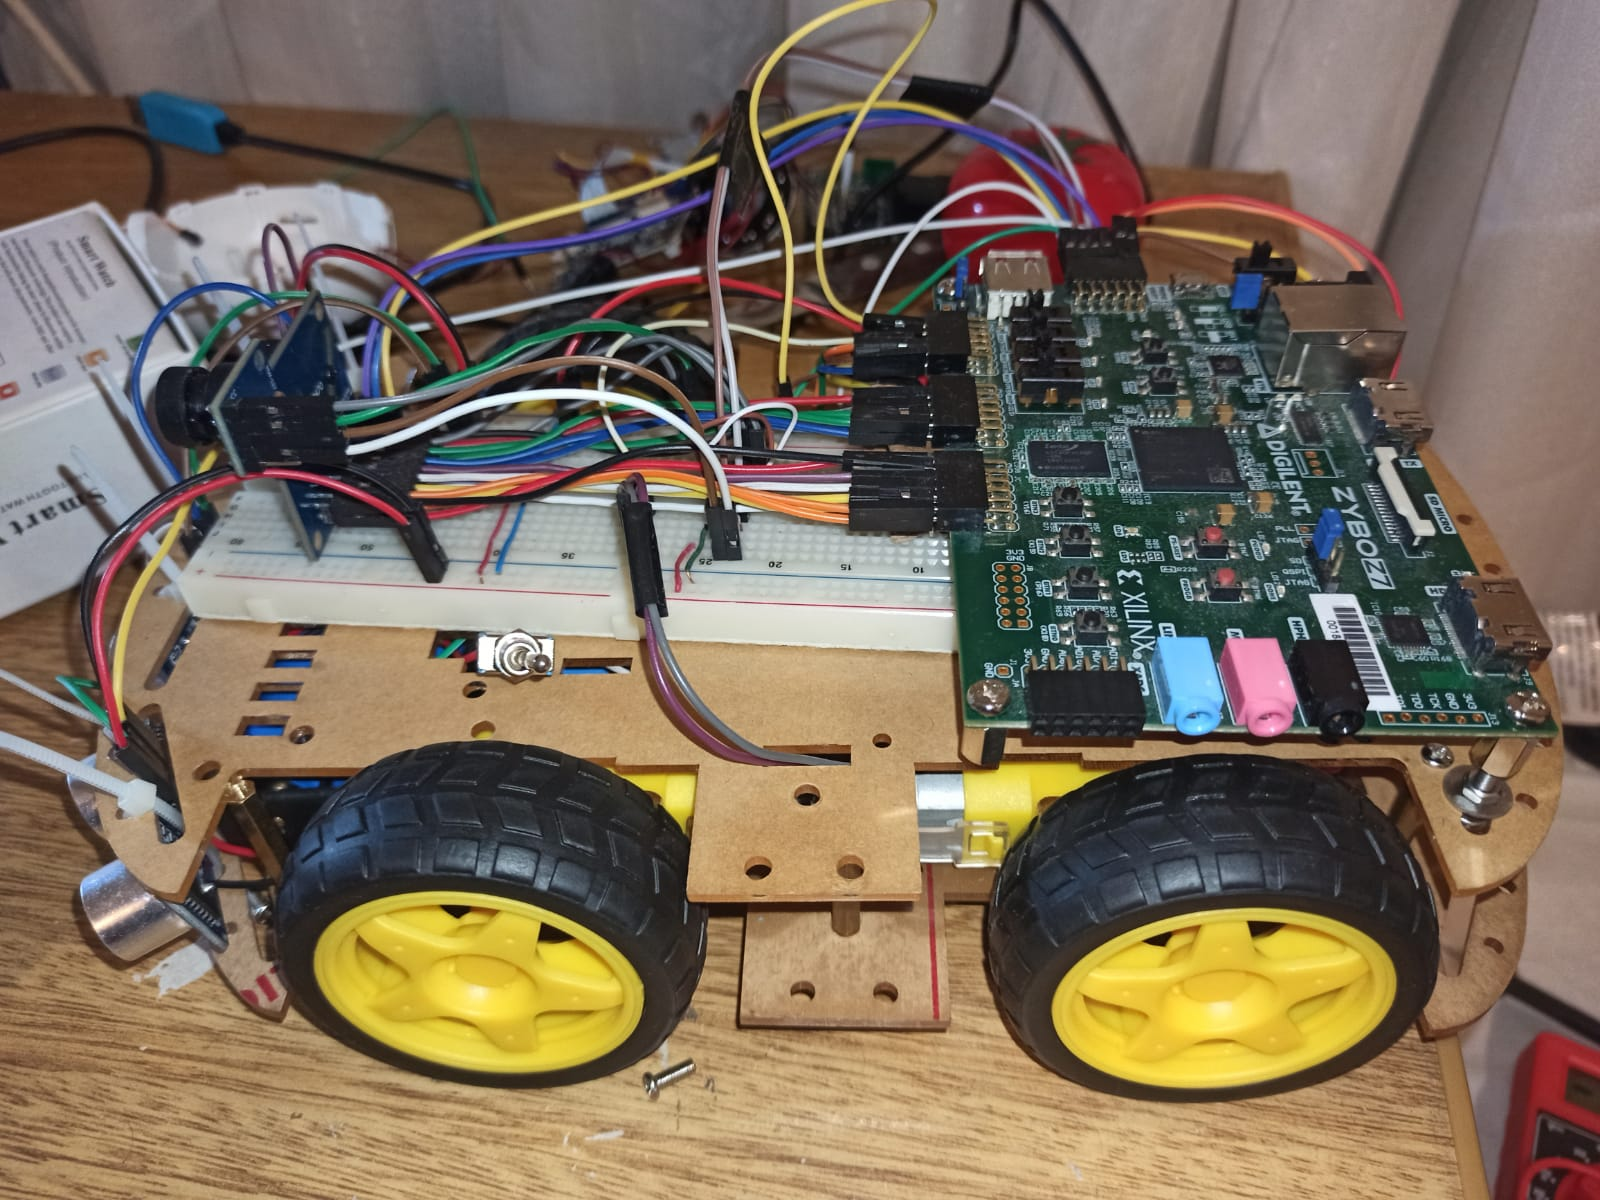
\includegraphics[height=1.5in]{Tesis/Capitulos/05_CAPITULO_3/img/state10.jpeg}
%\caption{fig2}
\end{minipage}%
}%
\quad
\subfigure[Estado 6]{
\begin{minipage}[t]{0.35\linewidth}
\centering
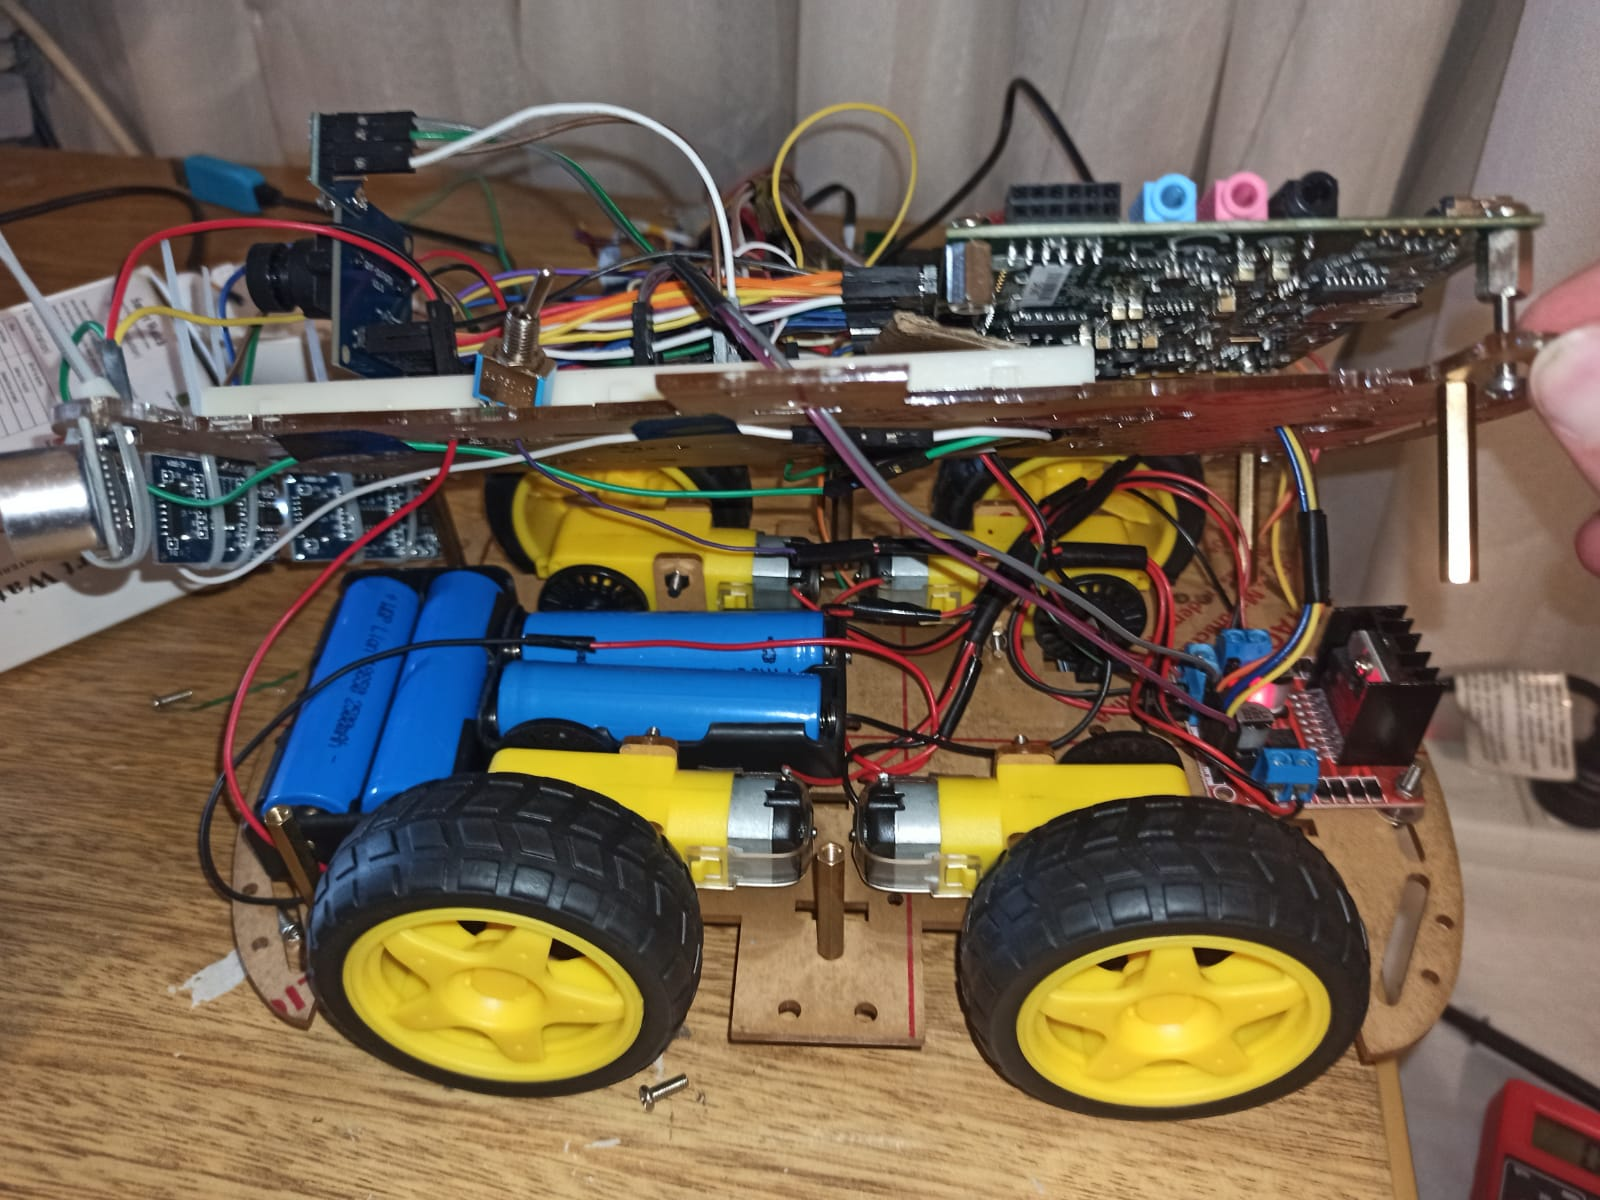
\includegraphics[height=1.5in]{Tesis/Capitulos/05_CAPITULO_3/img/state8.jpeg}
%\caption{fig2}
\end{minipage}%
}%
\centering
\caption{Elementos y hardware}
\end{figure}

\subsection{Diagrama en bloques del hardware}

\begin{center}
    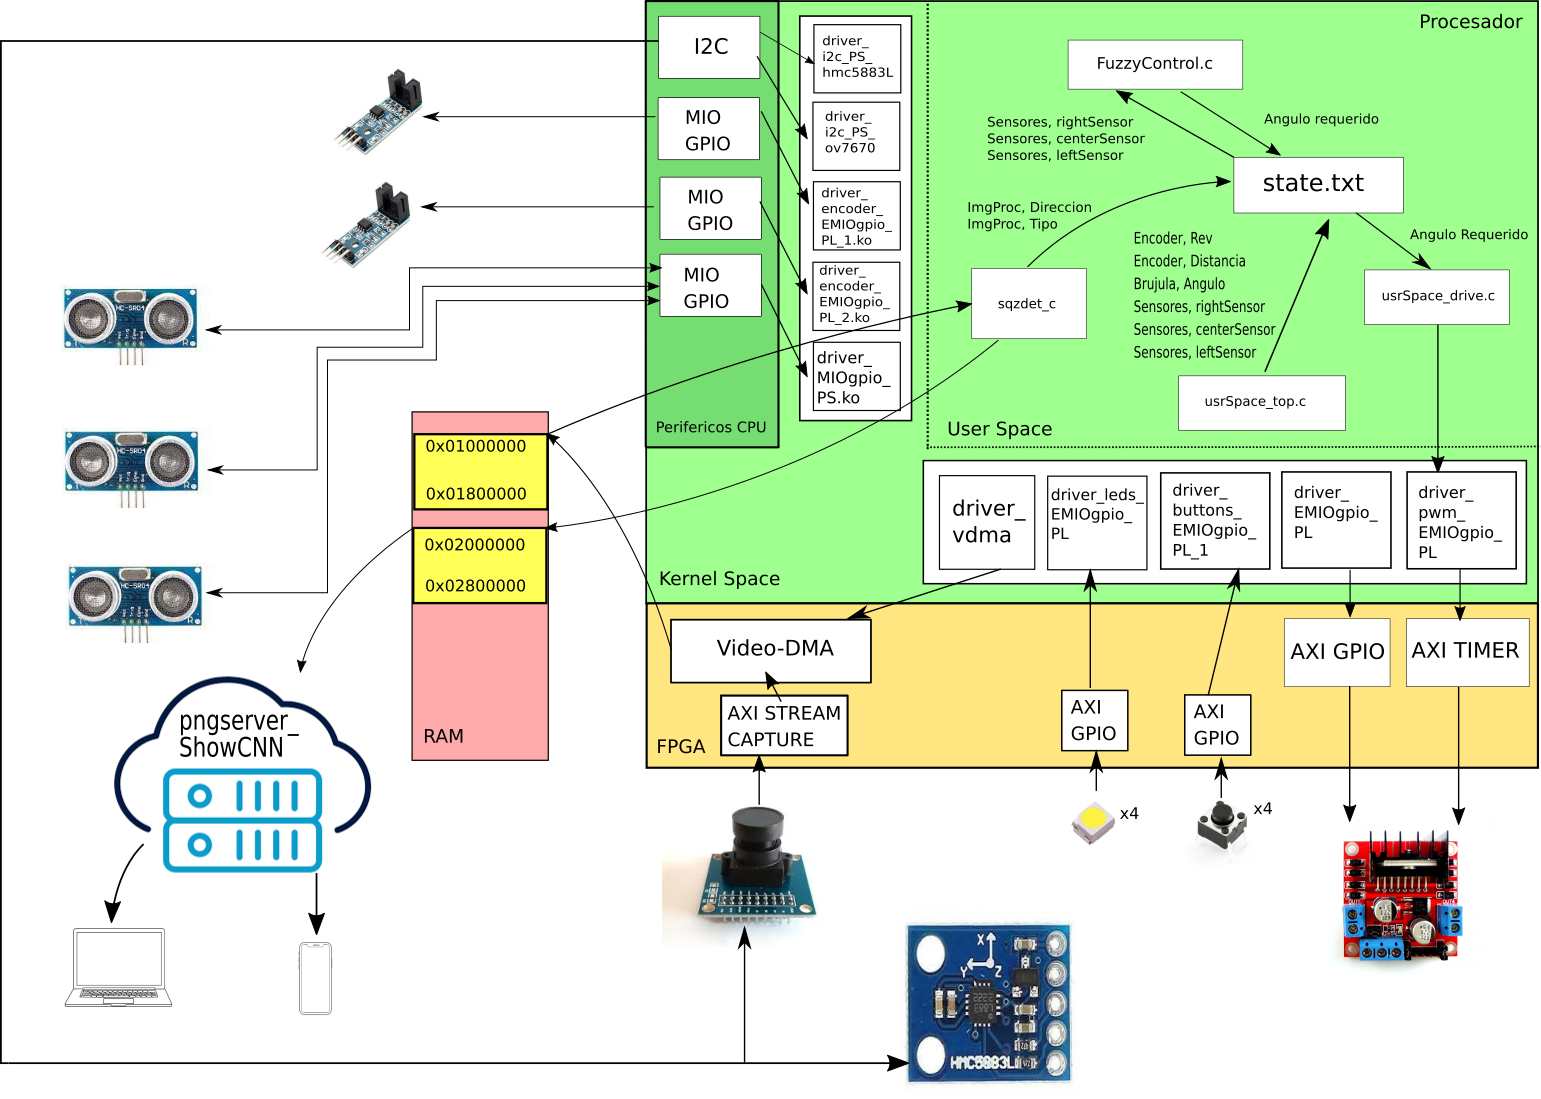
\includegraphics[scale=0.3]{Tesis/Capitulos/05_CAPITULO_3/BlockDiagram.png}
    \captionof{figure}{Diagrama en bloques}
\end{center}

\subsection{Drivers}

\subsection{Aplicaciones}

\subsection{Diagrama en bloques del sistema de control}